\chapter{Bayesian characterisation of postembryonic CMZ activity}
\label{chap:CMZ}
\section*{Synopsis}
\textit{(1) Variability in CMZ RPC population sizes and whole retinal volume estimates is better modelled Log-Normally than Normally. (2) The dynamics of CMZ RPC population measurements over the first year of life suggest that CMZ RPCs may be passing through a succession of phases with different cell cycle and niche exit rates. (3) Whole-eye modelling of CMZ population and retinal volume estimates suggests that only two such phases are necessary to explain these dynamics. (4) Slice modelling of the CMZ population more successfully recapitulates data, and suggest there is no timing difference in proliferative schedule across the CMZ's dorso-ventral axis. (5) Modelling RPC dynamics with a single phase of decaying cycle rate and constant exit rate is a superior description to the 2-phase models; decay models also suggest that there is no dorso-ventral gradient of cell cycle and niche exit parameters. (6) Nowakowski-type modelling of cumulative thymidine analogue labelling gives overstated cycle rates, comparable to the defective whole-eye models, but confirm no dorso-ventral differences in these parameters. More accurate estimates can be obtained using cell-based slice modelling. (7) Cohorts of neurons contributed to the retina by the CMZ are divided among layers in fractions that remain stable over time; however, the neural fates specified vary over time. (8) Retinal neurons contributed by the CMZ are turned over by microglia at a rate too low to be detected in labelled cohorts. (9) Explaining postembryonic CMZ dynamics requires different models from proliferatively-restricted embryonic lineage simulation. Slice models allow abstraction of spatial complexity. (10) Many opportunities for improved slice modelling exist.}

\section{Independent Log-Normal modelling of CMZ parameters}
To take up the question of how CMZ RPC activity evolves over time, we measured CMZ and retinal parameters in histological studies of cryosections of zebrafish eyes harvested over the first year of the animal's life. The initial approach is to geometrically impute measurements whole-eye CMZ and retinal volume from sample central cryosections, calculated as described in \autoref{sec:lenspopest}. These derived measurements form the first dataset we consider.

While it remains common to assume that population census data are Normally distributed, it is been known \cite{Heath1967} that Log-Normal distributions are usually better models of the outcomes produced by additive processes with small, variable steps (like population sizes or income distributions). Since all of our models require modelling distributions of population data, we start by selecting the most explanatory population model.

As described in more detail in \autoref{ssec:NormalModels}, we conclude that population variability in CMZ census and retinal volume estimates are best described by independent Log-Normal distributions. Because Log-Normal distributions are simply transformed Normal Gaussian distributions, we may model our uncertainty about their parameters with Normal-Gamma distributions over the mean and variance of the underlying Normal distribution of the Log-Normal population model \cite{Murphy2007}. This is explained in more detail in \autoref{ssec:normalgamma}. A useful analytic feature of the Normal-Gamma prior is that the marginal posterior distribution of the mean, assuming an uninformative (ignorance) prior, is a location-scaled T distribution. Most of the descriptive statistics in the next section, therefore, calculate the 95\% credible interval for the posterior mean of the underlying by T distributions (with the correct change of variables by exponential transformation to produce the features of the correct Log-Normal distribution). Unfortunately, differences of T distributions are not, themselves, necessarily T-distributed, so we have relied on Monte Carlo estimation of rates of change of the these posterior means over time. 

\section{Survey of CMZ population and gross retinal contribution}

If it is true that the majority of zebrafish retinogenesis occurs postembryonically, and that models trained on embryonic data do not describe this period well, as seen in \autoref{chap:SMME}, what characterises this CMZ-driven phase of retinogenesis? A schematic overview of the appearance of the CMZ during the first three months of post-embryonic life is presented in \autoref{cmz_dev_schematic}, displaying the progressive expansion of the neural retina and the relative size of the CMZ over this time period.

\begin{figure}[!h]
    \makebox[\textwidth][c]{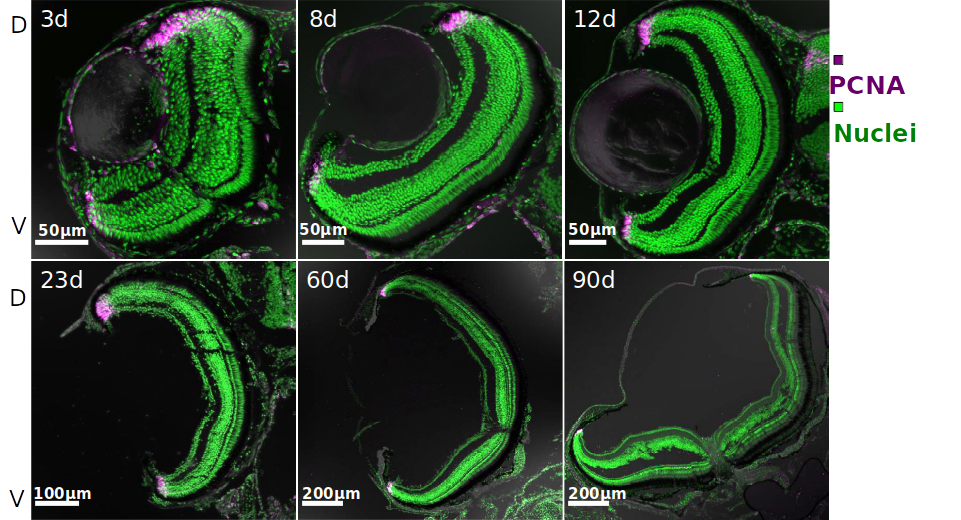
\includegraphics[width=1.1\textwidth]{cmz/cmz_schematic.png}}    
    \caption{{\bf Micrographic overview of CMZ development in \textit{D.rerio}, 3-90dpf}}
    Representative confocal micrograph maximum intensity projections (MIPs) of \SI{14}{\micro\metre} coronal eye cryosections, processed via IHC, of zebrafish of noted ages. Magenta – anti-PCNA staining. Green – Hoechst 33342 nuclear staining. Note changing scale bars.
    \label{cmz_dev_schematic}
    Methods in \autoref{ssec:PCNA}.
\end{figure}

We first estimate mean CMZ annulus population and retinal volume over the first year of life, in \autoref{CMZoverall}, panels A and C. The lack of growth observed in the first week of life suggests an initial quiescent period in the population history of the CMZ. Observations in \autoref{rysCMZontogeny}, showing CMZ RPCs are proliferating too slowly to be labelled by a 12 hour pulse of a thymidine analogue at 10dpf in the siblings of npat mutants, also suggest this quiescence. On the other hand, we have good confidence that retinal volume continues to grow over this time; 99.56\% of the marginal posterior mass of the mean 5dpf estimate is above the 3dpf mean, which may indicate any proliferative pause is too short to appear in the retinal volume data.

\begin{figure}[!h]
    \makebox[\textwidth][c]{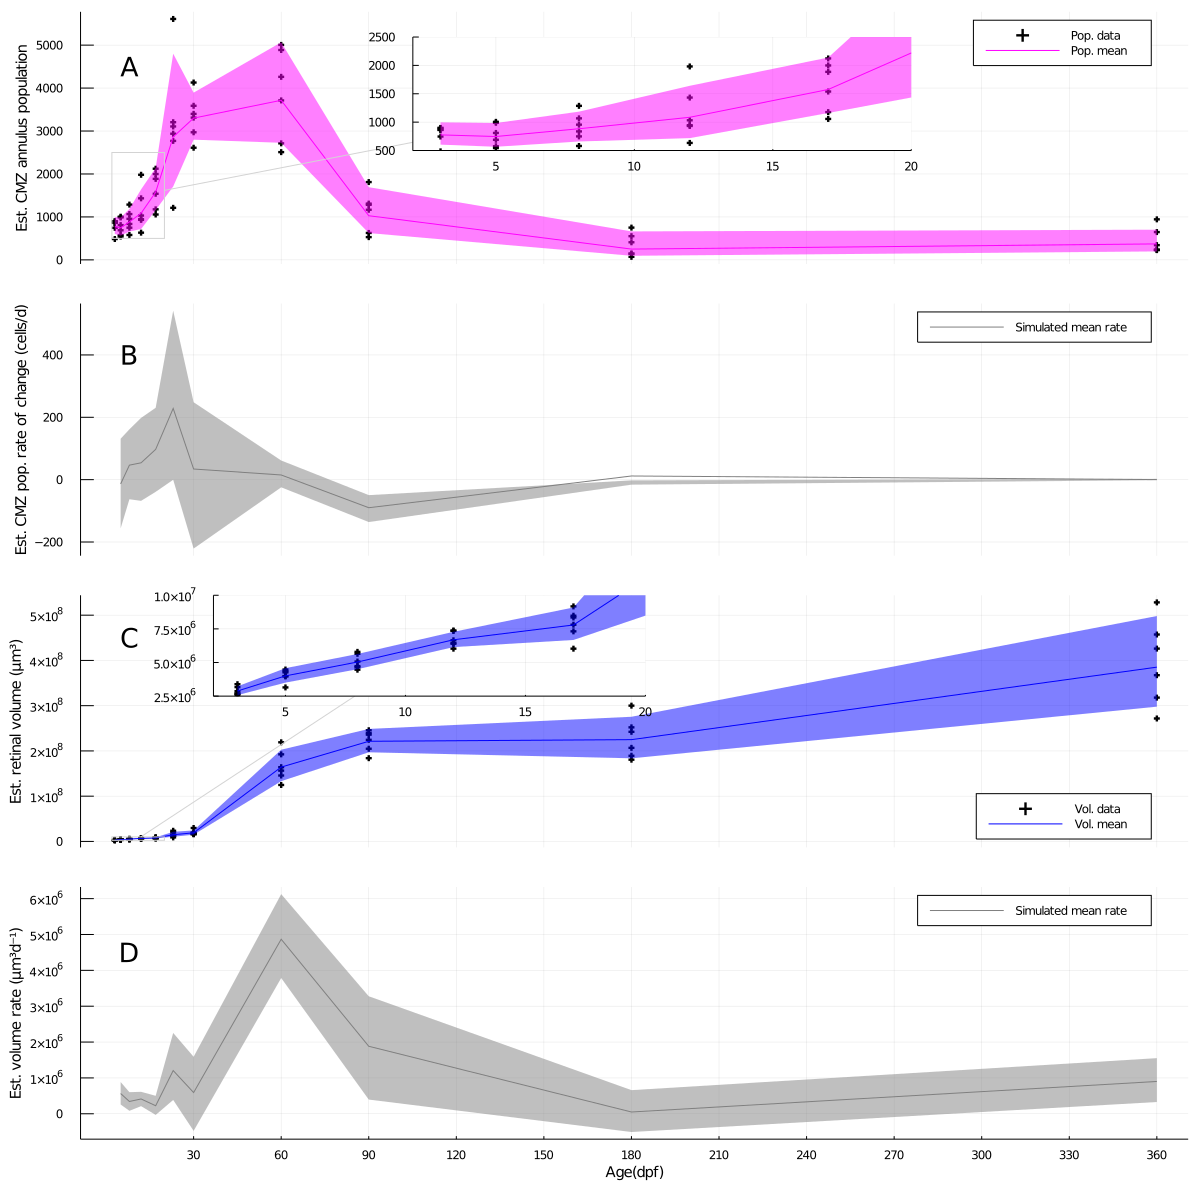
\includegraphics[width=1.\textwidth]{cmz/CMZoverall.png}}    
    \caption{{\bf Population and activity of the CMZ over the first year of \textit{D.rerio} life}}
    Panel A: Marginal posterior mean CMZ annulus population. Panel B: Marginal posterior mean retinal volume estimate. Insets in Panels A \& B display data from 3-17 dpf. Panel C: Marginal posterior mean of the proliferative index of the CMZ annulus, assayed by specified retinal neurons with incorporated thymidine from an 8hr pulse at the indicated ages. Panel D: Mean daily rate of volumetric increase of the neural retina, calculated as the difference in volumes between two ages over the number of elapsed days. All means are displayed in a band representing the $\pm 95 \%$ credible interval for the marginal posterior distribution of the mean.
    \label{CMZoverall}
    Methods in \autoref{ssec:CMZpopvolest}, \autoref{ssec:MCrates}.
    Code in \autoref{ssec:a10popsurvey}.
\end{figure}

The first two to three weeks of life (magnified in lens insets in panels A and C) see a slow build in both estimated CMZ annulus population and retinal volume compared to the large increase which follows. While zebrafish are better staged by size than age \cite{Parichy2009}, the onset of this growth seems to come earlier than the metamorphic transition from larval to juvenile stages at ~45dpf \cite{Singleman2014}. This raises the question of how the CMZ contributes to the retina during the critical period of exponential growth of the organism, between about 45 and 90dpf. It is plausible, for instance, that the growth of the CMZ population mainly reflects the increased cell cycle rate, with RPCs specifying at some steady rate, or that the CMZ builds itself up for a wave of increased niche exit and specification somewhat later, similarly to the sequence of events in the embryonic central retina.

To ascertain this timing, we simulated the mean daily rate of change of the CMZ annulus population and retinal volume, by performing Monte Carlo difference operations between samples from the marginal posterior means of subsequent timepoints. These simulated mean rates and their associated, empirically determined confidence intervals are plotted in \autoref{CMZoverall} panels B and D. These show the time-structure of the phenomenon; the increase in simulated daily CMZ population growth rate occurs before the increase in retinal volume, but the CMZ population estimate does not begin to drop off until 60dpf, by which time the majority of volumetric growth is complete. This seems to substantiate some combination of the scenarios outlined above: there is an early buildup of CMZ population around 18-30dpf, before CMZ RPCs begin to make their primary contribution to the retina between 30-60dpf, which seems to be characterised by much slower population growth and more rapid volumetric growth, implying steady and elevated specification and niche exit of RPCs. 

Subsequent to the bulk of the CMZ buildup and contribution to the retina, the population of the CMZ declines at about 39\% the rate of its peak ascent, with an estimated -90.1$\frac{cells}{d}$ by 90dpf. This thins out the CMZ population to below its inital value, spread out over a much larger peripheral annulus, for a much less dense mature CMZ. Interestingly, the 95\% CI on the marginal posterior mean of estimated retinal volume at 180 dpf (ranging from \SI{1.84E8}{\cubic\micro\metre} to \SI{2.75E8}{\cubic\micro\metre}) completely encompasses the 95\% CI on volume at 90dpf (\SI{1.96E8}{\cubic\micro\metre}-\SI{2.48E8}{\cubic\micro\metre}), while the 360dpf mean (\SI{3.85E8}{\cubic\micro\metre}) is greater than six standard deviations from the 180dpf mean (\SI{2.25E8}{\cubic\micro\metre}). This suggests a possible second period of quiescence from approximately 90-180dpf, followed by steady contribution to the retina without a buildup in the CMZ population subsequently.

Given this description, the ontogeny of the CMZ as a stem cell niche could be well-described by different phases of activity, with different rates of proliferation and specification. It is not immediately clear what sort of periodization is justified by the data. It seems plausible that as few as two phases could explain the data well enough: an initial phase of logarithmic growth, with short cell cycle time and lower exit rate of RPCs from the CMZ into the specified neural retina, followed by a second phase of decay with longer cycle time and higher exit rate. On the other hand, perhaps some of the data features noted above justify a more complex model that captures, for instance, the initial quiescent period, or the post-180dpf growth of the retina. Because this is a question of how much model structure is justified by our data, we may address it as a model selection problem.

\section{Two-phase periodization of postembryonic CMZ activity by phased difference equation modelling}
\label{sec:phaseGMC}
To perform our model selection task, we simulate the time-evolution of CMZ population and retinal volume. This requires initial values for the size of the simulated CMZ populations and the volumes of the simulated retinae they are associated with. Given the findings presented in \autoref{gausscorrelation}, we are justified in initializing CMZ population and retinal volume by independent samples from the Log-Normal models of their interindividual variability at 3dpf, the end of embryogenesis and the beginning of the period of CMZ-driven retinal growth. To produce new, simulated values of CMZ population and retinal volume, we apply a system of difference equations as follows, where $pop_n$ is the population at $n$ dpf, $CT$ is the mean cell cycle time of the population in hours, and $\epsilon$ is the proportion of the population at time $n-1$ that exits cycle and contributes to the volume of the specified neural retina, and $\mu_{cv}$ is the mean volume per cell contributed to the retina in \si{\cubic\micro\metre}:

\begin{equation}
    p_n=p_{n-1} \cdot 2^{\frac{24}{CT}} - p_{n-1} \cdot \epsilon
    \label{popeq}
\end{equation}

\begin{equation}
    v_n=v_{n-1} + p_{n-1} \cdot \epsilon \cdot \mu_{cv}
    \label{voleq}
\end{equation}

A model "phase" can then be defined by the $CT$ and $\epsilon$ parameters it applies to update the population and volume, over the appropriate number of days. The full parameterisation of a model with $p$ phases is given by $p$ pairs of $CT$ and $\epsilon$ values, and $p-1$ phase transition dates. $\mu_{cv}$, which is taken to apply equally to all phases, is estimated from 3 dpf nuclear measurements, as described in \autoref{ssec:CMZpopvolest}. This model is described further in \autoref{sec:CMZmodel}.

Given an initial population and volume sampled from the Log-Normal models of their interindividual distributions, \autoref{popeq} and \autoref{voleq} are be applied to these values to produce simulated sample measurements. Many such samples obtained by \hyperref[ssec:MonteCarlo]{Monte Carlo} can be used to estimate Log-Normal distributions for simulated CMZ populations and retinal volume, which can be used to score the model against observations. By defining prior distributions over the model parameters, we may sample from the prior to initialize a model ensemble. The ensemble can then be compressed by \hyperref[ssec:nested]{nested sampling}, moving each model-particle over the parameter space by Galilean Monte Carlo, as described in \autoref{ssec:GMC}. Using typical procedures applied in nested sampling \cite{Skilling2006}, we estimated the Bayesian evidence, maximum a posteriori model output, and marginal posterior distributions on parameters for 2 and 3-phase models.

\begin{figure}[!h]
    \makebox[\textwidth][c]{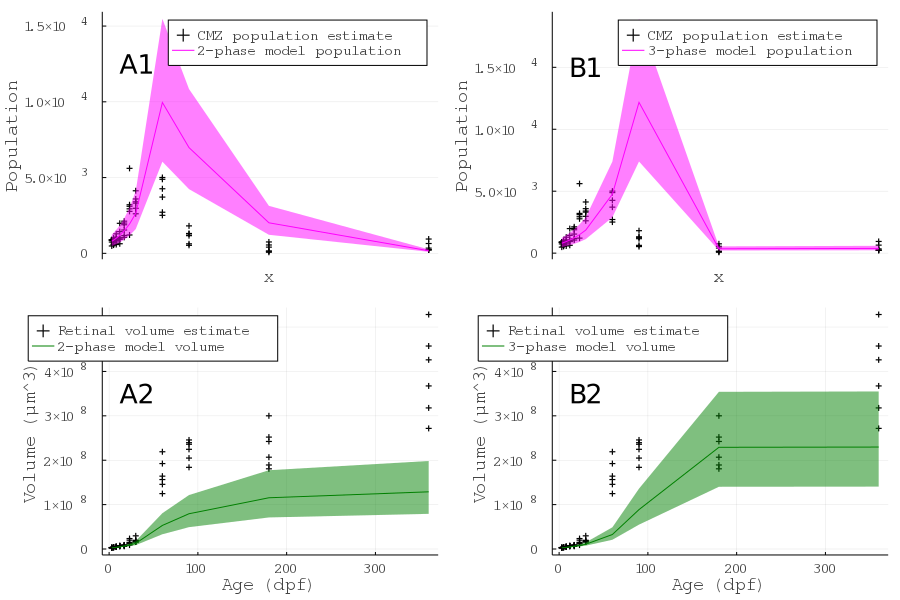
\includegraphics[width=1.2\textwidth]{cmz/a10pMAP.png}}    
    \caption{{\bf Maximum a posteriori output of periodization models}}
    \label{phaseMAPout}
    Population and volume estimates from observations (crosses) plotted with mean $\pm$ 95\% probability density model output, for the 2-phase model (A panels) and 3-phase model (B panels). A1,B1: population estimates. A2,B2: volume estimates. Insets provide magnified views of data from the first 30dpf.
    Methods in \autoref{ssec:GMCev}.
    Code in \autoref{ssec:a10periodisation}.
\end{figure}

The maximum a posteriori model output shows the major problem with this simple model; the model relationship between changes in CMZ population and changes in volume breaks down rapidly. That is, the later volume estimates are too large for the CMZ to produce, given the calculated cellular volume ($\mu_{cv}$) at 3dpf. The models fit the early population and volume data better, but the population peak is dragged upward to produce more-likely volume output at later ages. While it is possible that the later CMZ contributes more volume per neuron to the cellular retina, it seems more likely that the volume approximation applies better to more-nearly spherical eyes at younger ages, than to the flattened eyes of later ages. When we tried floating $\mu_{cv}$ as a variable within the model, the MAP results were similar (data not shown), suggesting that a constant value for $\mu_{cv}$ across ages is the problem in achieving good model fits, not the particular value chosen. This reinforces the idea that the problem relates to the breakdown of the retinal volume estimate at later ages.

While this limitation prevents either model from explaining the combined estimate datasets very well, they are in this sense under the same constraint, and so some inference about the number of phases justified by the data is still possible. Evidence estimates for the 2-phase and 3-phase models, given these data, are presented in \autoref{phasetable}. There are greater than 3500 orders of magnitude more evidence for the 2-phase model; this result has over 200 standard deviations of significance. This reflects the expanded parameter space in the 3-phase model, which has 8 parameters, compared to the 2-phase models' 5. The additional flexibility afforded by the 3rd phase in fitting the later volume data is unable to overcome the evidentiary penalty associated with the larger parameter space. We conclude that the 2-phase model is a better-justified description of these data.

\begin{table}[!ht]
    \centering
    \caption{{\bf Evidence favours a 2-phase periodization of CMZ activity}}
    \begin{tabular}{|l|l|l|l|} \hline 
        {\bf 2-phase logZ} & {\bf 3-phase logZ} & {\bf logZR} & {\bf $\sigma$ Significance}\\ \hline
        \textbf{-7147.3 ± 9.4} & -10743.0 ± 13.0 & 3596.0 ± 16.0 & 227.624\\ \hline
        \end{tabular}
    \begin{flushleft} logZ: logarithm of p(D), the marginal likelihood of the data, or model evidence. logZR: evidence ratio; positive ratios in favour of the 2-phase model. Largest evidence value bolded.
    Methods in \autoref{ssec:GMCev}.
    Code in \autoref{ssec:a10periodisation}.
    \end{flushleft}
    \label{phasetable}
\end{table}

While the parameter estimates associated with these models are clearly unreliable, they are useful to inspect in for comparison to the simulations to follow. We present the parameterization of the MAP model output displayed above in \autoref{phaseMAPtable}. Unsurprisingly, the selected 2-phase model begins with a first phase of rapid proliferation, with a $CT$ of 14.5 hr, followed by a second, slower phase of 17.5 hr. The imputed exit rate $\epsilon$ is greater than 200\% of the day's starting population in the first phase, suggesting that new cells exit the CMZ after about 12 hours, around one cycle, while the second phase exit rate is lower, with 160\% of the day's starting population exiting the CMZ, again suggesting a residency time of about one cycle. The imputed phase transition age is about 23dpf. Due to the volume estimate problem noted above, it is reasonable to believe that the $CT$ estimates are likely too short, the $\epsilon$ estimates too high, all favoured in order to produce higher volume estimates at later ages.

\begin{table}[!ht]
    \centering
    \caption{{\bf Maximum a posteriori parameter estimates for periodization models}}
    \begin{tabular}{|l|l|l|}
        \hline
        {\bf Parameter} & {\bf 2-phase MAP} & {\bf 3-phase MAP}\\ \hline
        Phase 1 $CT$ (h) & 14.5 & 14.9\\ \hline\
        Phase 1 $\epsilon$ & 2.02 & 1.95\\ \hline
        Phase 2 $CT$ (h) & 17.5 & 75.6\\ \hline
        Phase 2 $\epsilon$ & 1.6 & 0.29\\ \hline
        Phase 3 $CT$ (h) & NA & 68.4\\ \hline
        Phase 3 $\epsilon$ & NA & 0.27\\ \hline
        Transition 1 age & 23.2 & 47.9\\ \hline
        Transition 2 age & NA & 179.4\\ \hline
    \end{tabular}
    \begin{flushleft}
        $CT$: cycle time.
        $\epsilon$: niche exit rate.
        Methods in \autoref{ssec:GMCev}.
        Code in \autoref{ssec:a10periodisation}.    
    \end{flushleft}
    \label{phaseMAPtable}
\end{table}

Because nested sampling produces weighted samples from the posterior, we can estimate posterior distributions on parameters. We did so by kernel density estimation, to investigate whether the marginal posterior distributions for the selected model are polymodal. This can reveal how the evidence supports multiple hypotheses about the parameters of the two imputed phases. Kernel density estimates (KDEs) for marginal posterior distributions on the 2-phase models' parameters are presented in \autoref{phasemarginals}. 

These estimates reveal monomodal posterior distributions over the parameters. $CT$ posteriors are well constrained to a small part of the sampling space (left panels, X axes, and top right panel), with the MAP parameter estimates given in \autoref{phaseMAPtable} falling within the most dense regions. However, it is evident that the data do not constrain phase exit rates $\epsilon$ (left panels, Y axes) very well. That is, the marginal posterior probability distributions for these parameters are very widely spread.  The marginal posterior distribution on the age at which the transition between phases occurs is plotted in the bottom right of \autoref{phasemarginals}; the KDE suggests that the age of phase transition is likely around 23 dpf.

\begin{figure}[!h]
    \makebox[\textwidth][c]{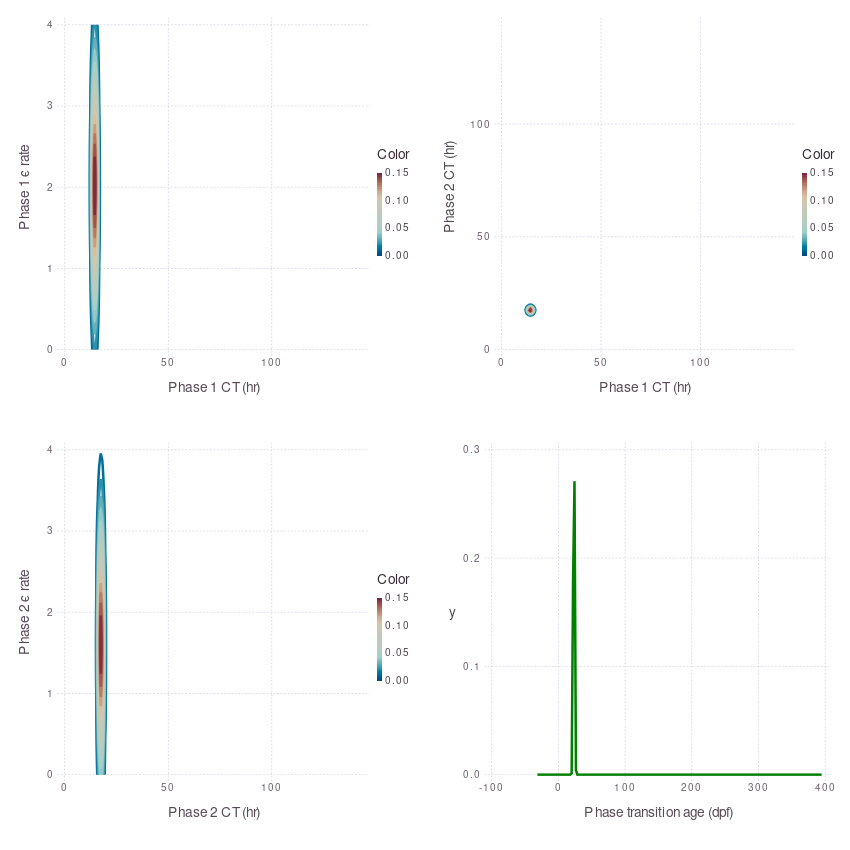
\includegraphics[width=.8\textwidth]{cmz/a10pmarginals.png}}    
    \caption{{\bf Kernel density estimates of marginal posterior parameter distributions, 2-phase model}}
    Prior distributions (magenta) apply to parameters of both phases. Maximum a posteriori model parameterisation indicated by vertical lines.
    Panel A: Marginal posterior distributions on Phase 1 and 2 $CT$ cycle time parameters. 
    Panel B: Marginal posterior distributions on Phase 1 and 2 $\epsilon$ niche exit rate parameters.
    Panel C: Marginal posterior distribution on Phase 1 to 2 transition age parameter.
    \label{phasemarginals}
    Methods in \autoref{ssec:GMCkde}.
    Code in \autoref{ssec:a10periodisation}.    
\end{figure}

The lower exit rate associated with MAP second phase highlights the fact that the relative cycle time or exit rate between phases is irrelevant to the overall behaviour of the system. What matters is whether the cycle time and exit rate within a phase produce a growing or shrinking CMZ. We conclude that, while our global model of CMZ population and volumetric retinal contribution is too flawed to make good parameter estimates, a 2-phase model of this activity is better substantiated by the evidence than a 3-phase model. We proceed on this basis, tentatively accepting the 2-phase model, and taking up the idea of the "slice model" introduced in \autoref{ssec:slice}, to investigate modelling the CMZ RPC population more concretely, directly from sectional observations, rather than from the calculated population and retinal volume estimates presented above.

\FloatBarrier

\section{Phased slice-models of CMZ population dynamics suggest subtle shifts across stable-population contour}
\label{sec:sliceGMC}

In the course of the preceding investigations, it became apparent that the CMZ population asymmetry mentioned in \autoref{chap:SMMEoutro} was not a static phenomenon, with the dorsal lobe of the CMZ annulus being consistently more populous than the ventral lobe, as generally implied by the sources covered in \autoref{chap:RPCreview}. Rather, both the extent and orientation of asymmetry change over time. Sectional population totals for the dorsal and ventral CMZ are presented in \autoref{DVontology}, Panel A, alongside the related intra-individual asymmetry ratio in Panel B. The initially pronounced dorsal population and reduced ventral population both seem to go through the overall boom-bust progression of CMZ population, but their relative proportion within individuals reverses itself over the period from 17-90dpf. We also observed a similar phenomenon occurring across the naso-temporal axis over the same time period (\autoref{NTontology}).

\begin{figure}[!h]
    \makebox[\textwidth][c]{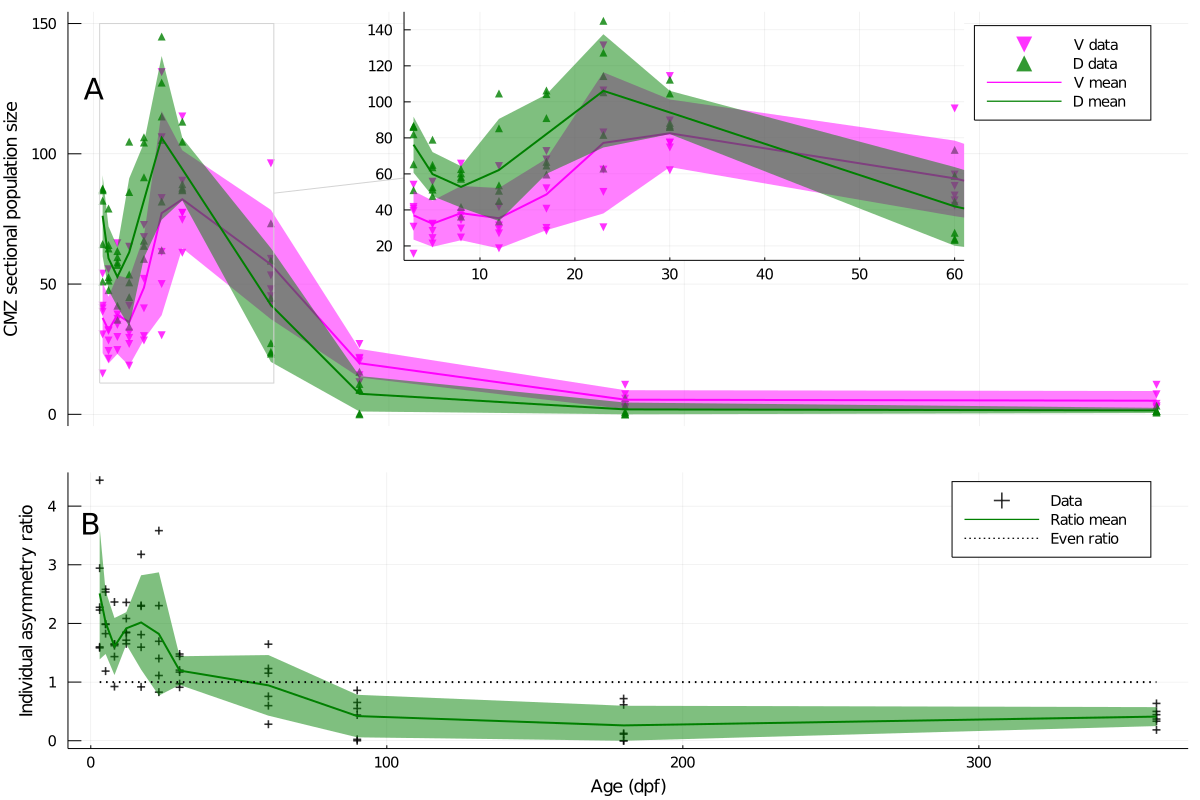
\includegraphics[width=1.2\textwidth]{cmz/DVontology.png}}    
    \caption{{\bf Developmental progression of dorso-ventral population asymmetry in the CMZ.}}
    Marginal posterior distribution of mean dorsal (D) and ventral (V) population size in 14$\mu$m coronal cryosections (panel A) or intra-individual D/V count asymmetry ratio (panel B), $\pm 95\%$ credible interval, n=5 animals per age. Data points represent mean counts from three central sections of an experimental animal's eye. 
    \label{DVontology}
    Methods in \autoref{ssec:PCNA}.
    Code in \autoref{ssec:a10dvratio}. 
\end{figure}

Inspected closely, these data provide a possible rationale for the reversal of asymmetry in the proliferative dynamics of the niche itself: the sectional (or ``slice'') population of the dorsal CMZ is increasing beyond its postembryonic minimum by 12dpf, while the ventral CMZ takes until 17dpf to exhibit a noticeable increase in size; moreover, the peak dorsal population is achieved by 23dpf, whilst ventrally the peak is only achieved at 30dpf. This suggests that the dorsal and ventral CMZ populations may undergo similar, time-shifted processes of proliferation from different starting populations. If this is so, an explanation for this time-shifted phenomenon could have fundamental relevance to predicting and controlling the proliferative behaviour of peripheral RPCs and stem cells.

To test this hypothesis, we used a ``slice model'' of the CMZ, where the thickness of the slice is taken to be the same as the observed cryosection thickness (\SI{14}{\micro\metre}). The population of the CMZ is modelled with a difference equation, as above, but with an additional exit term representing lateral, circumferential contributions of the CMZ to the generation of new, adjacent ``slices''. The value of this term is calculated from the difference in CMZ annulus diameter over the calculated time period, as implied by a power-law model of lens growth fitted to observations, discussed in \autoref{sec:lenspopest}. The resultant difference equation is \autoref{sliceeq}. Terms are as defined above, except that $p_n$ is the sectional population at $n$ dpf, and not the total CMZ annulus population; additionally, $\eta$ is defined as the daily circumferential exit rate implied by the power-law model. The model is detailed in \autoref{sec:slicemodel}.

\begin{equation}
    p_n=p_{n-1} \cdot 2^{\frac{24}{CT}} - p_{n-1} \cdot \epsilon - \eta
    \label{sliceeq}
\end{equation}

We reasoned that, if the phase transition occurs earlier in the dorsal CMZ than in the ventral CMZ, there should be some informational gain in separating these observations vs. both slices being governed by one model. We therefore estimated the evidence, MAP, and posterior marginals for 2-phase models given the sectional dorsal and ventral populations, both combined and as separately-parameterised slices. To focus on the most informative subset of the data for our hypothesis, we restricted this analysis to the population data within the first three months of life.

The slice model proves to have greater success at explaining sectional counts than the whole-eye model does at explaining the annulus population estimates; maximum a posteriori model output is presented in \autoref{dvMAPout}. In particular, all of the models adequately represent the early decline in sectional populations, arising from rapid early growth of the eye that exceeds the CMZs' proliferative capacity, without further ado; there is no justification for a separate early quiescent period, as suggested above.

\begin{figure}[!h]
    \makebox[\textwidth][c]{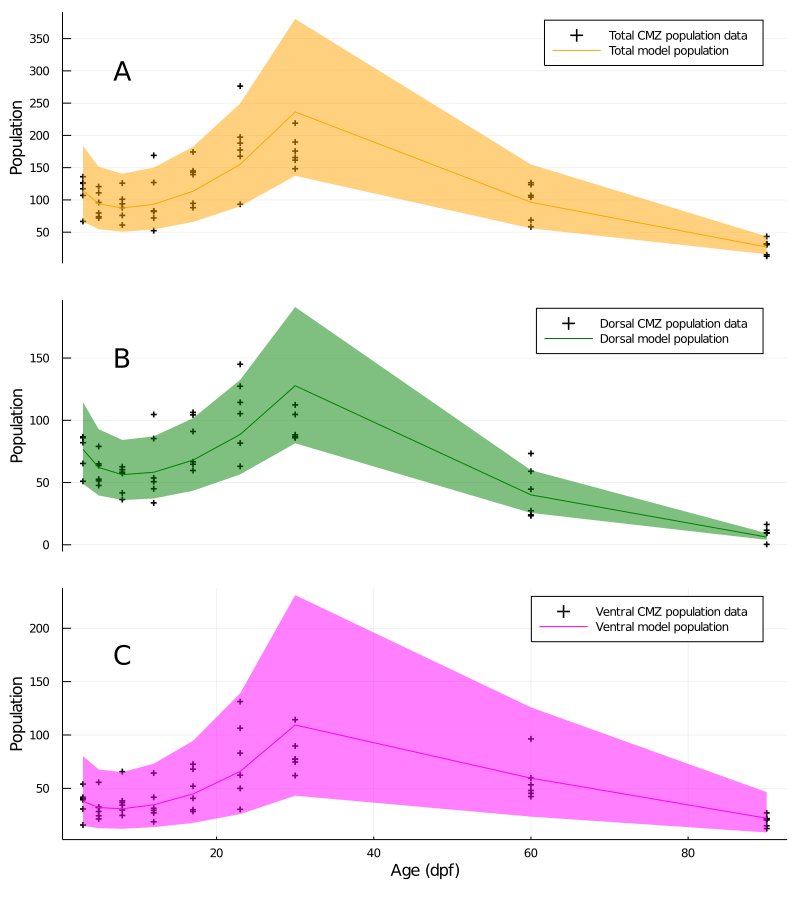
\includegraphics[width=1.0\textwidth]{cmz/a10dvMAP.png}}    
    \caption{{\bf Maximum a posteriori output of total, dorsal, and ventral CMZ slice models}}
    \label{dvMAPout}
    Population and volume estimates from observations (crosses) plotted with mean $\pm$ 95\% probability density model output, for the total CMZ population model (panels A \& B), dorsal CMZ population model (panel C), and ventral CMZ population model (panel D).
    Methods in \autoref{ssec:GMCev}.
    Code in \autoref{ssec:a10dvslice}. 
\end{figure}

The hypothesis that there is a time-shift in the phase transition across the dorso-ventral axis is not supported by these models. First, the evidence estimates demonstrate that we are not justified in separating the dorsal and ventral populations. The total-population slice model receives greater than 500 orders of magnitude more evidence than the joint evidence for the separate dorsal and ventral models, with greater than 20 standard deviations of significance, as displayed in \autoref{dvtable}. It is interesting to note that the evidence for the dorsal model (-579.9 ± 0.9) is substantially less than for the ventral model (-328.9 ± 0.5). This may indicate a causal influence on the dorsal population that is neither in the model nor acting on the ventral population, or it may be an uninformative sampling effect. A second indication that this hypothesis is unsupported are the MAP model parameter values, summarized in \autoref{dvMAPtable}. The dorsal MAP transition is actually later than the ventral date, which further suggests the original model-idea of a time-shifted late ventral phase change is unsupported by these data.

\begin{table}[!ht]
    \centering
    \caption{{\bf Evidence favours a combined slice model over separate dorsal and ventral models}}
    \begin{tabular}{|l|l|l|l|l|}
        \hline
        {\bf Combined D/V model logZ} & {\bf Separate D/V model logZ} & {\bf logZR} & {\bf $\sigma$ Significance}\\ \hline
        \textbf{-874.3 ± 1.2} & -908.8 ± 1.0 & 34.5 ± 1.6 & 21.9\\ \hline
    \end{tabular}
    \begin{flushleft} logZ: logarithm of p(D), the marginal likelihood of the data, or model evidence. logZR: evidence ratio; positive ratio in favour of the combined model. Largest evidence value bolded.
    Methods in \autoref{ssec:GMCev}.
    Code in \autoref{ssec:a10dvslice}.     
    \end{flushleft}
    \label{dvtable}
\end{table}

The MAP parameters for the combined slice model suggest that those found for the 2-phase MAP in \autoref{phasemarginals} overstate cell cycle speed and exit rate. The combined slice model gives $CT$s of 34.4 and 23.3 hours for the first and second phases, compared to 14.5 and 17.5 estimated for the whole-eye model. Moreover, the niche exit rates $\epsilon$ are estimated at .54 and 1.07 for the combined slice model, compared to 2.02 and 1.6 for the whole-eye model. The values of the slice model seem more realistic in general; it seems unlikely that over one day, fully 200\% of the day's starting CMZ population has exited the niche and entered the specified neural retina, for instance, as implied by the first phase exit rate of the whole-eye model. As well, given that $CT$ represents an average cycle time over a heterogenous population of progenitors, many of whom are becoming postmitotic, $CT$ values over 24 hr seem much more plausible than the ~15 hr parameter required for the whole-eye model to produce its unrealistically exaggerated population.

\begin{table}[!ht]
    \centering
    \caption{{\bf Maximum a posteriori parameter estimates for slice models}}
    \begin{tabular}{|l|l|l|l|}
        \hline
        {\bf Parameter} & {\bf Combined MAP} & {\bf Dorsal MAP} & {\bf Ventral MAP}\\ \hline
        Phase 1 $CT$ (h) & 34.4 & 33.6 & 17.8\\ \hline
        Phase 1 $\epsilon$ & 0.54 & 0.57 & 1.43\\ \hline
        Phase 2 $CT$ (h) & 23.3 & 35.0 & 11.2\\ \hline
        Phase 2 $\epsilon$ & 1.07 & 0.67 & 3.42\\ \hline
        Transition age & 32.2 & 41.0 & 27.8\\ \hline
        \end{tabular}
    \begin{flushleft}
        $CT$: cycle time.
        $\epsilon$: niche exit rate.
        Methods in \autoref{ssec:GMCev}.
        Code in \autoref{ssec:a10dvslice}.    
    \end{flushleft}
    \label{dvMAPtable}
\end{table}

The marginal posterior distributions of the total slice model, presented in \autoref{dvmarginals}, are substantially more polymodal than those in \autoref{phasemarginals}. This illustrates how data can support multiple hypotheses about model parameters to different degrees. When the phase marginal $CT$ and $\epsilon$ are plotted together, they display the characteristic density curves displayed in Panels A and B of \autoref{dvmarginals}. This supplies the most interesting information available by estimating this slice model. Firstly, the posterior marginal distributions of the first and second phase are very close to one another. Importantly, when the $CT$-$\epsilon$ contour which gives a stable population is plotted (dotted lines), it becomes obvious that the bulk of the first phase posterior lies just under this curve, while the bulk of the second phase lies just above it. This strongly suggests that the population dynamics of the CMZ may be characterised by a relatively subtle shift across the stable population contour, rather than distinct phases.

It should be noted that the MAP estimate does not occupy the most credible KDE kernel. An important property of nested sampling is that the accuracy of evidence calculations is traded off against the accuracy of estimating the posterior distribution \cite{Speagle2019}, as noted in \autoref{ssec:GMC}. Since we have here prioritized evidence estimation, this is one cause of this discrepancy; the MAP models themselves may have relatively little weight in the KDE estimates. The oversampling of the prior periphery noted in \autoref{chap:GMC}, as well as the very significant polymodality of the model posteriors displayed in Supplementary \autoref{polymodality} also contribute to this problem\footnote{A more conventional approach to reporting posterior estimates is to provide the mean and variance of the distribution, rather than the position of the most likely model in the MAP ensemble. We have eschewed this because of the tendency of \path{GMC_NS} to oversample the prior volume.}.

\begin{figure}[!h]
    \makebox[\textwidth][c]{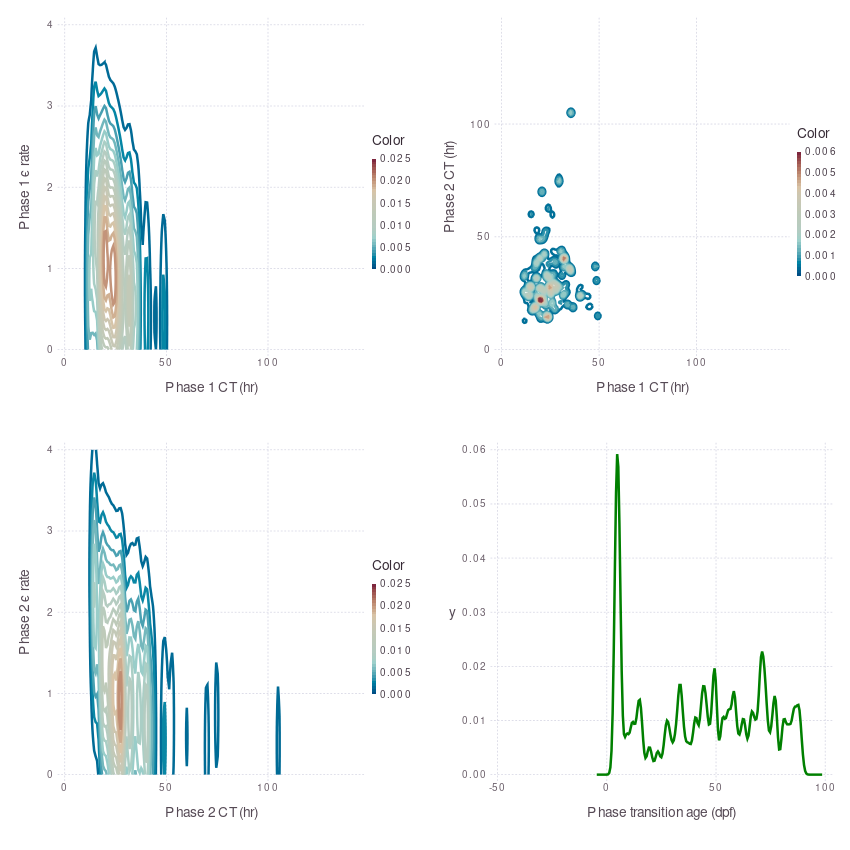
\includegraphics[width=1.\textwidth]{cmz/a10dvmarginals.png}}    
    \caption{{\bf Kernel density estimates of marginal posterior parameter distributions, total slice model}}
    Panel A: Bivariate KDE of Phase 1 posterior $CT$ vs. $\epsilon$ density. Univariate marginals, with priors, are plotted to the left and below of the bivariate panel.

    Panel B: Bivariate KDE of Phase 2 posterior $CT$ vs. $\epsilon$ density. Univariate marginals, with priors, are plotted to the left and below of the bivariate panel.

    Panel C: Univariate KDE of Phase 1-2 transition age.

    Line height (univariate panels) or color scale (bivariate panels) indicates the estimated marginal posterior density present at the indicated parameter value. MAP parameters are given with magenta crosses (bivariate panels).
    \label{dvmarginals}
    Methods in \autoref{ssec:GMCkde}.
    Code in \autoref{ssec:a10dvslice}.    
\end{figure}

On the basis of the marginal posterior analysis of this model, we suspected that separately parameterised phases is not the best available description of the data. In particular, the relatively small shifts across the balanced population contour implied by the posterior distributions argues strongly for a model with one phase with a slowly decaying cycle rate.

\FloatBarrier

\section{Slice models of decaying cell cycle support anatomical homogeneity of RPC behaviour}
\label{sec:decaymodel}

To model the CMZ as a population of cells with a continuously lengthening cell cycle time, we modify the slice model described above by removing the phases and introducing an exponential decay equation for cycle time. This results in a slice model with three parameters: the initial cycle time ($CT_{i}$), a constant exit rate ($\epsilon$), and a decay constant ($\kappa$). Population values are updated daily as per \autoref{sliceeq}, including the use of the lens model, except that the cycle time $t$ days after initialising is determined by $CT_{t}=CT_{i} \cdot e^{\kappa \cdot t}$. More detail is provided in \autoref{sec:decaymodel}

\begin{figure}[!h]
    \makebox[\textwidth][c]{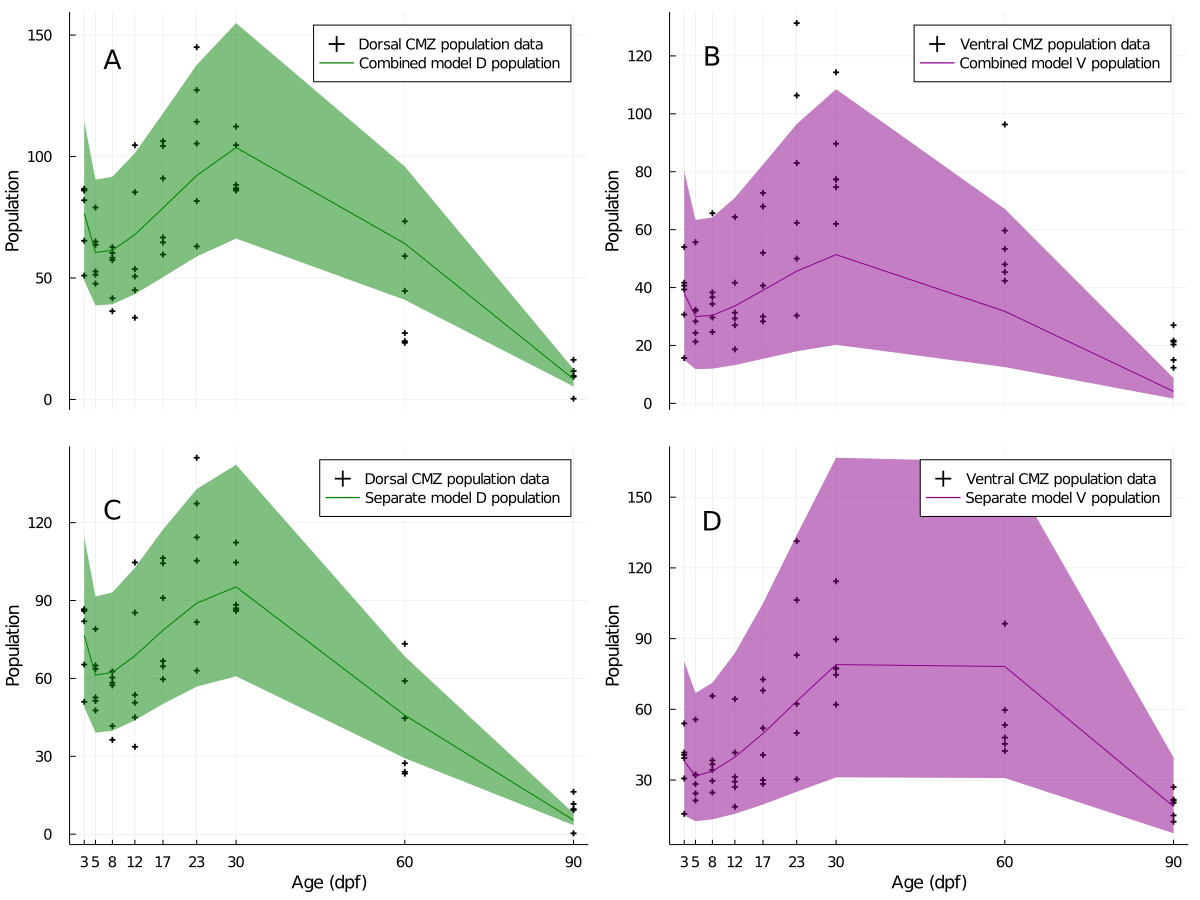
\includegraphics[width=1.0\textwidth]{cmz/a10dvdecayMAP.png}}    
    \caption{{\bf Maximum a posteriori output of total, dorsal, and ventral CMZ decay models}}
    \label{decayMAPoutput}
    Population and volume estimates from observations (crosses) plotted with mean $\pm$ 95\% probability density model output, for the total CMZ population model (panel A \& B), dorsal CMZ population model (panel C), and ventral CMZ population model (panel D).
    Methods in \autoref{ssec:GMCev}.
    Code in \autoref{ssec:a10dvdecayslice}. 
\end{figure}

We performed the same sampling routine on the same 3-90dpf dataset used for the earlier slice models, to enable direct comparison between them. The evidence calculations are presented in \autoref{decayevtable}. The combined decay model substantially outperforms the combined slice model selected above, as well as separate decay models. Therefore, the model evidence supports the use of the decay model for describing RPC behaviour in general; however, there is insufficient evidence to distinguish between dorsal and ventral populations using this model.

\begin{table}[!ht]
    \centering
    \caption{{\bf Evidence supports separate dorsal and ventral decay models}}
    \begin{tabular}{|l|l|l|l|l|l|}
        \hline
        {\bf Combined slice logZ} & {\bf Combined decay logZ} & {\bf D/V decay logZ} & {\bf decay logZR} & {\bf $\sigma$ Sig.}\\ \hline
        -874.3 ± 1.2 & {\bf -762.6 ± 0.7} & -794.6 ± 0.8 & 32.0 ± 1.1 & 29.3\\ \hline
    \end{tabular}
    \begin{flushleft} logZ: logarithm of p(D), the marginal likelihood of the data, or model evidence. logZR: evidence ratio between separate D/V decay models and a combined decay model; positive ratio in favour of the combined model. Combined slice model from \autoref{dvtable} included in left column for comparison. Largest evidence value bolded.
    Methods in \autoref{ssec:GMCev}.
    Code in \autoref{ssec:a10dvdecayslice}.     
    \end{flushleft}
    \label{decayevtable}
\end{table}

MAP model output for the combined and separate decay models is presented in \autoref{decayMAPoutput}, while the MAP parameter estimates are summarised in \autoref{decayMAPtable}. Generally speaking, the values estimated for the parameters of the decay model suggest a much gentler proliferative schedule for RPCs, with initial cycle times measured in days, and daily niche exit rates of between 15-30\% of the RPC population. Cumulative thymidine analogue labelling results, presented below, suggest these values are unrealistically long. Interestingly, MAP parameterisations for the split Dorsal and Ventral models do not imply that dorsal RPCs are more active than those found ventrally. Probably, if consistent regional biases in CMZ RPC behaviour exist, better data would be required to constrain niche exit rate. Indeed, it seems likely that the lack of effective constraint on the model's niche exit rate $\epsilon$ allows for the unrealistically long $CT_{i}$ suggested by both combined and separate decay models. We conclude that explanations invoking differences in CMZ RPC behaviour across morphological axes  cannot be supported with our models and datasets, indicating that morphological homogeneity of these parameters is descriptively adequate at this level.

\begin{table}[!ht]
    \centering
    \caption{{\bf Maximum a posteriori parameter estimates for decay models}}
    \begin{tabular}{|l|l|l|l|}
        \hline
        {\bf Parameter} & {\bf Combined MAP} & {\bf Dorsal MAP} & {\bf Ventral MAP}\\ \hline
        $CT_{i}$ (h) & 52.0 & 69.7 & 62.1\\ \hline
        $\kappa$ decay& 0.0067 & 0.0124 & 0.0091\\ \hline
        $\epsilon$ exit& 0.276 & 0.164 & 0.189\\ \hline
    \end{tabular}
    \begin{flushleft}
        $CT_{i}$: Initial cycle time.
        $\kappa$: Exponential cycle time decay constant.
        $\epsilon$: niche exit rate.
        Methods in \autoref{ssec:GMCev}.
        Code in \autoref{ssec:a10dvdecayslice}.    
    \end{flushleft}
    \label{decayMAPtable}
\end{table}

Marginal distributions on these parameters are summarised in \autoref{decaymarginals}. We again note that the data are informative for parameters of cell cycle ($CT_{i}$ and $\kappa$), but give little information regarding niche exit rate. The MAP models found by GMC are well outside the kernel density estimates of the posterior distributions supplied by nested sampling this model. It is not clear why this should consistently be the case. The decay model may be characterised by small, high credibility modes that are outside the bulk of the less credible posterior mass; possibly, these are underweighted if they come late in the nested sampling process. In any case, the posterior marginals seem to confirm that there is little reason to separately distinguish dorsal and ventral subpopulations of CMZ RPCs.

\begin{figure}[!h]
    \makebox[\textwidth][c]{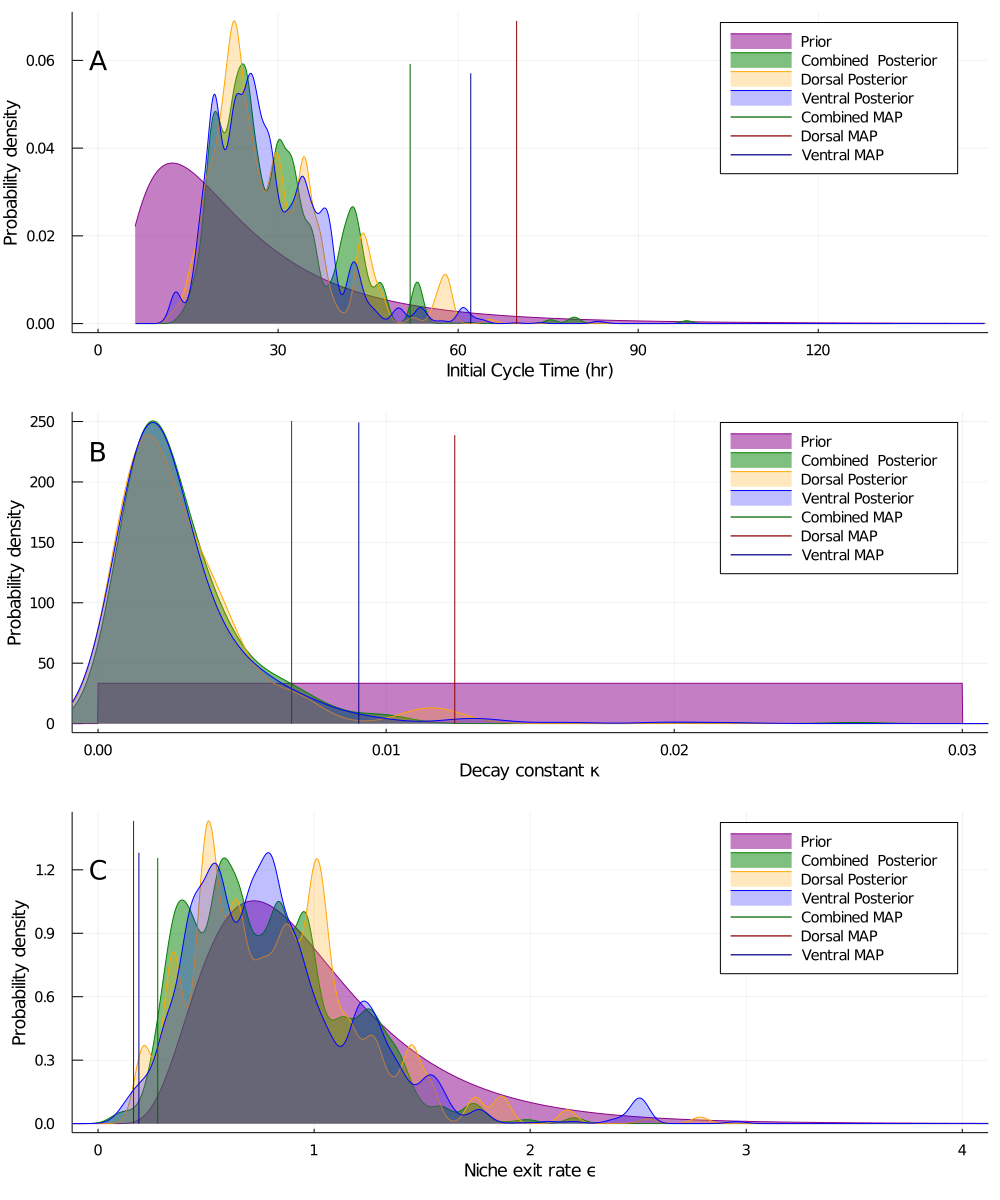
\includegraphics[width=.8\textwidth]{cmz/a10decaymarg.png}}    
    \caption{{\bf Kernel density estimates of marginal posterior parameter distributions, decay models}}
    \label{decaymarginals}

    Panel A: Marginal prior and posterior distributions on $CT_{i}$.
    Panel B: Marginal prior and posterior distributions on $\kappa$.
    Panel C: Marginal prior and posterior distributions on $\epsilon$.

    MAP model parameters are given by vertical lines.
    Methods in \autoref{ssec:GMCkde}.
    Code in \autoref{ssec:a10dvdecayslice}.    
\end{figure}

\FloatBarrier

\section{Bayesian inference of cycle parameters from cumulative thymidine labelling experiments supports slice model cycle time estimates}
\label{ssec:CMZcumedu}

We sought to confirm the plausibility of the $CT$ estimates obtained from modelling CMZ population measurements with an independent line of evidence. We  examined 3dpf CMZ RPCs cumulatively labelled with a 10.5 hour pulse of the thymidine analogue EdU \cite{Chehrehasa2009}. We used the Empirical Bayes approach to estimate the evidence for separate Nowakowski-style \cite{Nowakowski1989} linear models for the dorsal and ventral CMZ, against a model for both subpopulations combined. While this model is inadequate for reasons outlined in \autoref{chap:SMME}, it can serve to substantiate the first phase cycle time parameter. These results are summarized in \autoref{cumEdUtable}, with the relevant linear regressions displayed in Supplementary \autoref{cumEdUlinreg}.

\begin{table}[!ht]
    \centering
    \caption{{\bf Evidence favours whole-CMZ linear cycle models over separate D/V models}}
    \begin{tabular}{|l|l|l|l|} 
        \hline {\bf Model} & {\bf Implied $T_c$ (hr)} & {\bf Implied $T_s$ (hr)} & {\bf logZ}\\ \hline 
        Dorsal & 14.7 $\pm$ 1.6 & 1.38 $\pm$ 0.76 & 7.778\\ \hline 
        Ventral & 14.0 $\pm$ 1.2 & 0.8 $\pm$ 0.58 & 15.202\\ \hline
        Combined & 14.6 $\pm$ 1.1 & 1.25 $\pm$ 0.53 & {\bf26.165}\\ \hline
    \end{tabular}
   
    \begin{flushleft} $T_c$: calculated cell cycle time. $T_s$: calculated s-phase length. logZ: logarithm of p(D), the marginal likelihood of the data, or model evidence.  Largest evidence value bolded.
    Methods in \autoref{ssec:CMZEmpBayes}.
    Code in \autoref{ssec:a25dvlinreg}.    

    \end{flushleft}
    \label{cumEdUtable}
\end{table}

Firstly, there are approximately 3 orders of magnitude of evidence in favour of the combined model vs. the joint evidence for separate models (ie. 26.165 vs. 22.980). In general, this suggests that there is little traction to be gained by separating these observations along the D/V axis. The Nowakowski-calculated cell cycle time $T_c$ for the combined model, 14.6 $\pm$ 1.1 hr, includes the whole-eye MAP first phase $TC$, 14.5 hr, within one standard deviation. This suggests the Nowakowski model has similar problems to the whole-eye models presented in \autoref{phaseMAPout}, substantially overstating cycle rate. Calculated S phase lengths are also unrealistically short. Finally, the data seem to diverge from a linear trend toward the end of the pulse (see \autoref{cumEdUlinreg}), showing the limitations of this model.

Because the Nowakowski model is clearly inadequate for estimating RPC cycle parameters in the CMZ, we implemented a cell-based cycle simulator, similar to those in \autoref{chap:SMME}, to model discrete cumulative thymidine labelling counts, in lineages with explicitly simulated cycle events. This model is described further in \autoref{sec:thymidinemodel}. The MAP model output for this model is presented in \autoref{a25MAP}; it does a better job of describing the observations than the Nowakowski method, particularly at the earliest timepoints, due to simulation of cycle time correlation between sibling cells, as well as detector sensitivity. 

\begin{figure}[!h]
    \makebox[\textwidth][c]{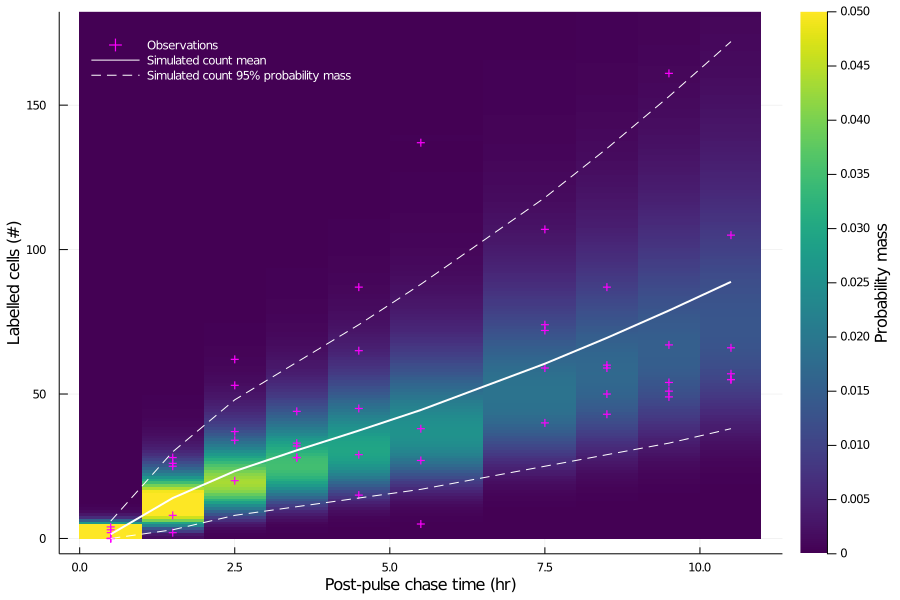
\includegraphics[width=1.\textwidth]{cmz/a25MAP.png}}    
    \caption{{\bf MAP model output and observations for thymidine slice model of 3dpf cumulative EdU labelling}}
    Count of EdU-positive cells observed in 14\si{\micro\metre} coronal cryosections through \textit{Danio} CMZs, at indicated chase times, during a 10 mM EdU pulse (magenta crosses), overlaid with MAP model output. Probability mass distribution of the discrete non-parametric output is shown by color scale; yellow values include counts with >.05 mass. Output mean and 95\% mass are indicated by solid and dashed white lines.

    Methods in \autoref{ssec:RyscumEdU}, \autoref{ssec:GMCev}. Code in \autoref{ssec:a25thymidinesim}.
    \label{a25MAP}
\end{figure}

KDE estimation of marginal distributions over the model parameters are presented in \autoref{a25marg}. These estimates give us a clear picture of what can be learnt from these data; mean cycle time and the length of S phase as a fraction of the cycle time are significantly compressed relative to the prior, but little can be gleaned about the variance of the cycle time distribution, and almost no information is available about the G1 or sister shift fraction. That is, for the parameters which the data offer little information, the posterior distribution correctly collapses back onto the prior, which indicates that this approach adequately copes with unconstrained parameters\footnote{The model is overparameterised relative to the available dataset. This was done deliberately to allow the model to be used with richer data than were available here; however, it does have the effect of making sampling against these observations less efficient than is achievable.}.

\begin{figure}[!h]
    \makebox[\textwidth][c]{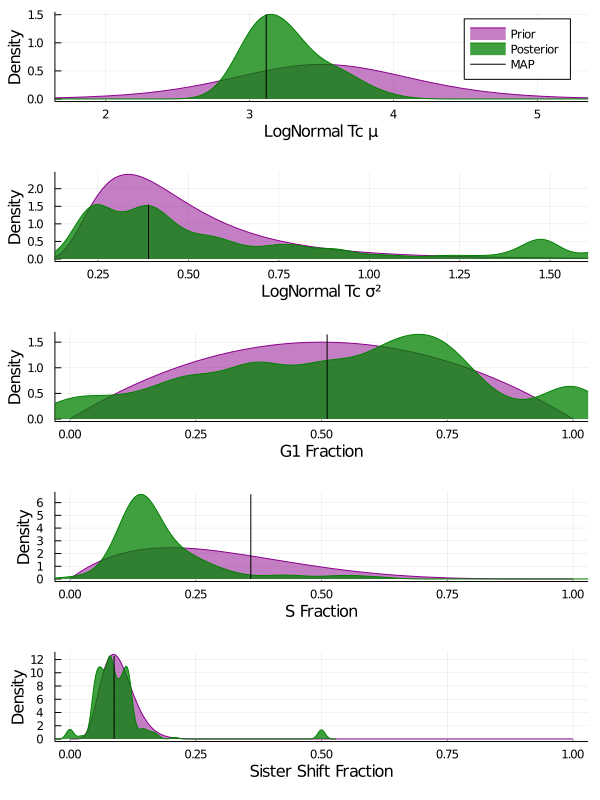
\includegraphics[width=.8\textwidth]{cmz/a25marginals.png}}    
    \caption{{\bf Marginal posterior distributions for thymidine slice model}}
    Marginal prior (magenta) and posterior (green) distributions on thymidine simulator cycle parameters, noted on the x axis. MAP model parameters are displayed with vertical black lines.

    Methods in \autoref{ssec:RyscumEdU}, \autoref{ssec:GMCkde}. Code in \autoref{ssec:a25thymidinesim}
    \label{a25marg}
\end{figure}

The MAP parameters for the LogNormal distribution of cycle times produces a mean cycle time of 24.0 hr. This seems to be a more realistic estimate of RPC cell cycle time, and tends to support the longer values estimated in the slice models, although it does suggest the 50+ hour $CT_{i}$ estimates for the decay models may be excessively long. Furthermore, this result supports our observation in \autoref{PerLineageFig} that the He model examined in \autoref{chap:SMME} substantially overstates the per-lineage proliferative rate of RPCs, at least in the CMZ; the He model's mean cycle time of 6 hours is much too fast to correctly model this population. It is likely that most reports of similar, very short cycle times for embryonic RPCs are underestimates of the actual distribution of cycle times.

Because the thymidine simulator's output resembles observations more closely than the Nowakowski model, produces more realistic parameter estimates than it, and clearly conveys how much information is available in the dataset, we suggest that this explicit simulation approach should be preferred to Nowakowski's method wherever the computational cost can be justified. 

\section{The CMZ contributes stably to each cellular layer with time-variable lineage composition}

By labelling CMZ RPCs with the thymidine analogue EdU in a pulse at 3, 23, and 90 dpf, followed by histochemical analysis for known zebrafish retinal neural lineage markers after a 7 day chase, we investigated the possibility that RPC lineage outcomes change over the life of the organism. This hypothesis is of particular interest, as differences in the mosaic organisation of embryonically-contributed central retina and CMZ-contributed peripheral retina remain unexplained \cite{Allison2010}. It may, moreover, have clinical significance, were quiescent peripheral stem cells to be entrained for regnerative medical purposes, as their lineage outcomes may be different than embryonic RPCs.  We used antibodies raised against Pax6 and Isl2b to mark retinal ganglion cells (RGCs) of the ganglion cell layer and amacrine cells of the inner nuclear layer. Anti-glutamine synthetase (GS) and anti-PKC$\beta$ were used to mark M\"{u}ller glia (MG) and bipolar cell (BPC) populations of the INL. The unique flattened nuclear morphology of horizontal neurons was used to identify them. Lastly, the antibody Zpr1, directed against an unknown antigen present in photoreceptors with double cone morphology, was used to mark these cells.

\begin{figure}[!h]
    \makebox[\textwidth][c]{\includegraphics[width=1.2\textwidth]{cmz/lineage.png}}    
    \caption{{\bf Representative 23dpf lineage marker confocal micrographs}}
    Panel A1: RGC/Amacrine staining group. A2: Isl2b channel. A3: Pax6 channel.

    Panel B1: MG/BPC staining group. B2: PKC$\beta$ channel. B3: GS channel.

    Panel C: Double cone staining group. Zpr1 channel.

    GCL: Ganglion cell layer. INL: Inner nuclear layer. ONL: Outer nuclear layer.
    Methods in \autoref{ssec:CMZlintrace}.
    \label{staininggroups}
\end{figure}

Observations were collected in "staining groups", which combined histological markers; representative confocal micrographs from this study in animals pulsed at 23dpf are displayed in \autoref{staininggroups}, while data from all ages are plotted in \autoref{layercontributions}.

\begin{figure}[!h]
    \makebox[\textwidth][c]{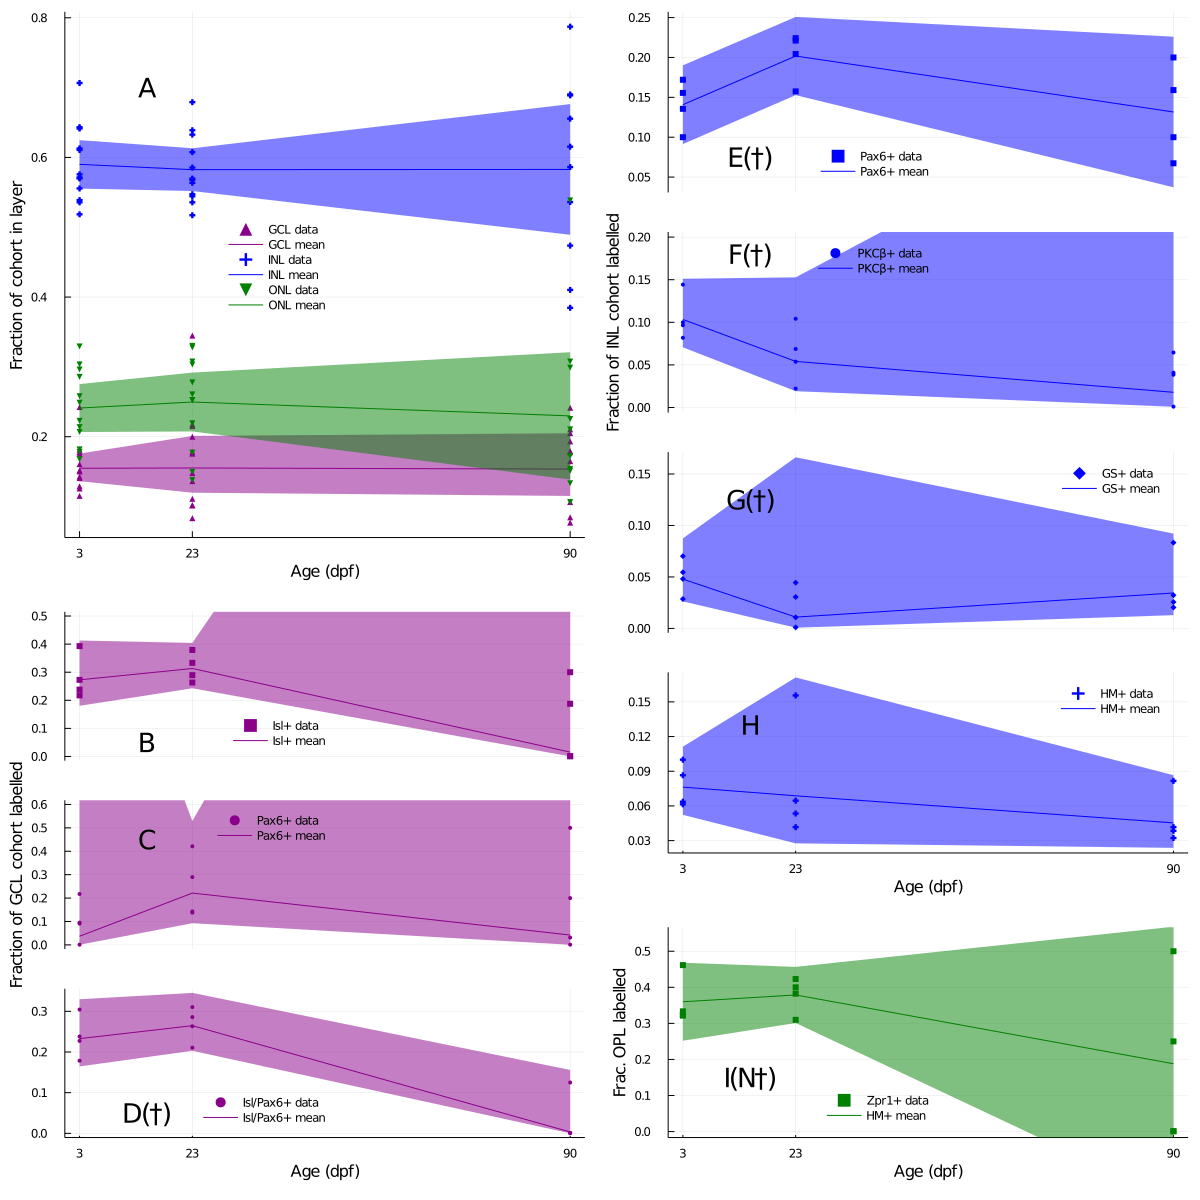
\includegraphics[width=1.2\textwidth]{cmz/layercontributions.png}}    
    \caption{{\bf Second-phase declines in CMZ-contributed Isl\/Pax6+ RGCs, PKC$\beta$+ bipolar neurons, and Zpr1+ double cones}}
    Overall fraction of CMZ-contributed cohort entering cellular layers (Panel A), or fraction of the layer subcohort expressing the noted immunohistochemical marker of lineage. All mean values are presented as marginal posterior means $\pm$ 95\%CI.

    $\lambda$: Fractional lineage contribution is modelled Log-Normally

    $\dagger$: Evidence supports time-varying model of fractional lineage contribution

    Magenta: GCL measurements; Blue: INL measurements; Green: ONL measurements

    Methods in \autoref{ssec:CMZlintrace}, \autoref{ssec:GMCev}.
    Code in \autoref{ssec:a19lineagetrace}.    
    \label{layercontributions}
\end{figure}

These data take the form of fractions of the thymidine-labelled cohort entering each of the three cellular layers (panel A of \autoref{layercontributions}), or the subfraction of the cohort within a given layer expressing a particular cellular marker (Panels B-I). While some variability is apparent in all of the measurements, it is unclear whether it is well-described as time-dependent in most cases. In order to address the question of whether CMZ layer or lineage outcomes differ over time, we needed to assess the joint evidence for separate models of each measurement at each age, against the evidence for a single model of the measurement for all of the assessed ages. 

Because it is not obvious that these fractional measurements are better described Log-Normally, as the underlying population counts are, we first assessed the joint evidence for Normal and Log-Normal models of the data, summarized in Supplementary \autoref{lineage_nlnev}. This supports Log-Normal modelling of all measurements aside from the INL and ONL overall fractions, as well as GCL-resident Pax6- and ONL-resident Zpr1-positive cells. We noted that the evidence estimates differs from the simple likelihood ratio tests in some cases, as summarized in Supplementary \autoref{lineage_lhratio}.  Without a clear fundamental justification for uniformly preferring one model or the other, we selected the best-supported model for each measurement. We estimated the evidence for an age-marginalized model, representing stable contribution to the layer or lineage over time, and compared this to the joint evidence for separate models at each age, representing a time-varying contribution model. These estimates are presented in \autoref{lineage_ev}.

\begin{table}[!ht]
    \caption{{\bf Evidence supports stable layer contributions with time-varying fate commitment}}
    \begin{tabular}{|l|l|l|l|l|l|l|} 
        \hline
        {\bf Layer} & {\bf Marker} & {\bf Cell type} & {\bf Stable logZ} & {\bf Time-vary logZ} & {\bf logZR} & {\bf $\sigma$ sign.}\\ \hline \hline
        GCL & Cohort & All GCL cells & {\bf -0.84 ± 0.71} & -30.96 ± 1.0 & 30.1 ± 1.2 & 24.7\\ \hline \hline
        GCL & Isl2b & RGC & -48.68 ± 0.26 & {\bf -23.76 ± 0.59} & -24.92 ± 0.64 & 39.0\\ \hline
        GCL & Pax6 & Displaced am. & {\bf -23.85 ± 0.44} & -40.08 ± 0.71 & 16.24 ± 0.84 & 19.3\\ \hline
        GCL & Isl2b/Pax6 & RGC subtype & -32.97 ± 0.28 & {\bf -16.82 ± 0.83} & -16.14 ± 0.87 & 18.5\\ \hline \hline
        INL & Cohort & All INL cells & {\bf -41.15 ± 0.49} & -52.65 ± 0.66 & 11.5 ± 0.82 & 14.0\\ \hline \hline
        INL & Pax6 & Amacrine cell & -15.37 ± 0.57 & {\bf -9.14 ± 0.46} & -6.23 ± 0.73 & 8.5\\ \hline
        INL & PKC$\beta$ & Bipolar cell & -5.99 ± 0.3 & {\bf 2.81 ± 0.54} & -8.79 ± 0.62 & 14.2\\ \hline
        INL & GS & M\"{u}ller glia & 14.34 ± 0.35 & {\bf 10.18 ± 0.6} & 4.17 ± 0.7 & 6.0\\ \hline
        INL & HM & Horizontal cell & {\bf 12.0 ± 0.31} &  3.02 ± 0.6 & 8.98 ± 0.68 & 13.3\\ \hline \hline
        ONL & Cohort & All ONL cells & {\bf -47.42 ± 0.45} & -63.19 ± 0.7 & 15.77 ± 0.83 & 19.1\\ \hline \hline
        ONL & Zpr1 & Double cones & {\bf -18.79 ± 0.37} & -31.63 ± 0.6 & 12.84 ± 0.7 & 18.3\\ \hline
    \end{tabular}
    \begin{flushleft}logZ: logarithm of p(D), the marginal likelihood of the data, or model evidence.  Largest evidence values bolded. logZR: evidence ratio; positive values in favour of stable model.
    Methods in \autoref{ssec:CMZlintrace}, \autoref{ssec:GMCev}.
    Code in \autoref{ssec:a19lineagetrace}.    
    \end{flushleft}
    \label{lineage_ev}
\end{table}

These calculations demonstrate that there is evidence for time-varying contributions to the retina, in particular, to RGC, amacrine, bipolar, and M{\"u}ller glial fates. All of these findings have between 6 and 39 standard deviations of significance. In the INL, the trend of the posterior mean for PKC$\beta$-positive bipolar neurons (panel F) and GS-positive M{\"u}ller glia of these lineages declines from the early postembryonic period (3dpf) to the late juvenile period (90dpf). Most of the time-varying fates show a downward trend in the fraction of the cohort expressing the relevant marker. These time-varying, declining lineages may be functionally related. However, we have no specific evidence that would implicate Isl2b/Pax6 double-positive RGCs in circuits with bipolar or amacrine cells, for instance. This nonetheless provides an explanation for the observation of a more-ordered retinal mosaic in later retinal contributions relative to the embryonic central remnant: since one or more sublineages in each layer are depleted in older fish, a different overall mosaic pattern as the neurons associate and pack together is expected. This may occur by changing the pattern of crystalline defects in this packing order, recently suggested as a mode of mosaic organisation \cite{Nunley2019}. Based on the timing of these changes, we tentatively ascribe this differential lineage production to the later phase of CMZ contribution, after the balance between proliferation and niche exit has shifted to the latter.

Lastly, we investigated the possibility that there might be detectable differences in layer or lineage contributions across the dorso-ventral axis; we tested this by measuring the evidence for age-marginalized combined models of fractional contribution against age-marginalized models split along the dorso-ventral axis. We found no evidence to support this hypothesis. These results are presented in Summary \autoref{lineage_dvev}.

\FloatBarrier

\section{Early retinal cohorts of the \textit{D. rerio} retina are turned over at a low rate by 4C4-positive microglia}
\label{sec:neuralfate}
Recently, extensive neural death has been reported in older zebrafish retinae \cite{Vanhoucke2018}. This was described as a ``neurodegenerative pathology" and suggested as a model of age-related neurodegeneration. However, during our thymidine analogue pulse-chase studies, CMZ-contributed cohorts often appeared less numerous only a month or two after their entry into the neural retina, even in juveniles of 30-90 days of age. Moreover, we observed numerous 4C4-positive microglia associating with the CMZ, as displayed in Supplementary \autoref{4C4micrograph}, which suggested that microglia may prune CMZ contributions. If neural retinal turnover occurs throughout the life of the organism, this would belie view that it should be treated as pathological, rather than constitutive. However, the thinning phenomenon could be explained by the changing morphology and geometry of the neural retina during this period. In particular, the neural retina thickens noticeably over this time, as displayed in Supplementary \autoref{morphology}. Although this increase is due, in large part, to the lengthening of photoreceptor outer segments, the inner nuclear layer is also significantly thickened. It is plausible that this process involves a compaction of the neurons along the coronal axis typically sampled, thus appearing to lose cells over time without this actually occurring. 

To investigate, we administered 24 hr pulses of EdU to 1dpf embryos, and followed with 24 hr pulses of BrdU at 23dpf to mark a CMZ-contributed cohort near the height of its activity. By taking both coronal and transverse sections through the eyes of animals at 30, 60, and 90 dpf, we sampled these cohorts from both morphological axes of the retina, and counted labelled sectional totals. Data were totalled across morphological axes to account for the possibility of the cohorts being compacted on the coronal plane and extended on the transverse one. In order to test the hypothesis of early turnover, we estimated the evidence for linearly correlated and uncorrelated models of cohort population over time, using the \hyperref[ssec:EmpiricalBayes]{Empirical Bayes} regression method. If the addition of a time-dependent term in the correlated regression model is justified by the evidence at these early ages, this supports the notion that \textit{D. rerio} retinal turnover is a lifelong phenomenon; if not, the apparent contraction of the cohorts is more likely a function of the alternative explanations noted above, or is occurring at too low a rate to be detected by these means. The results are summarized in \autoref{turnovertable}, with the regressions plotted in Supplementary \autoref{a27linreg}.

\begin{table}[!ht]
    \centering
    \caption{{\bf Evidence for linear regression models supports early cohort population stability}}
    \begin{tabular}{|l|l|l|l|}
    \hline
    {\bf Measurement} & {\bf Stable logZ} & {\bf Declining logZ} & {\bf logZR}\\ \hline
    1dpf Central Remnant & {\bf -212.953} & -214.167 & 1.213\\ \hline    
    30dpf Cohort & {\bf -107.567} & -110.827 & 3.261\\ \hline
    \end{tabular}
   
    \begin{flushleft}logZ: logarithm of p(D), the marginal likelihood of the data, or model evidence.  Largest evidence values bolded. logZR: evidence ratio; positive values in favour of stable model.
    Methods in \autoref{ssec:CMZEdU}, \autoref{ssec:CMZEmpBayes}.
    Code in \autoref{ssec:a27linreg}.
    \end{flushleft}
    \label{turnovertable}
\end{table}

There is more evidence for a model of cohort population that is stable over time than one correlated with time, indicating that the additional model complexity implied by allowing turnover is unjustified, for this early period. Despite this, we did find isolated instances where members of these cohorts were visibly being engulfed by 4C4-positive microglia; one such event is depicted in \autoref{CMZ4C4micrograph}. Moreover, we also observed TUNEL-positive nuclei in the central retina of \textit{rys} siblings in the early postembryonic period (\autoref{caspase}). This indicates that some level of turnover is occuring during this earlier period. The evidence ratio in favour of the uncorrelated models is not overwhelming, which suggests that the cohorts are not turned over at a high enough rate to be detectable in the early period, although the process does occur even at this early age. In order to confirm this finding, we estimated the evidence for age-marginalized Log-Normal models of the population counts against age-differentiated models, representing time-constant and time-varying population models. This investigation resolves any ambiguity: no time-varying model is justified by the available evidence, as summarized in \autoref{turnoverGMCtable}.

\begin{figure}[!h]
    \makebox[\textwidth][c]{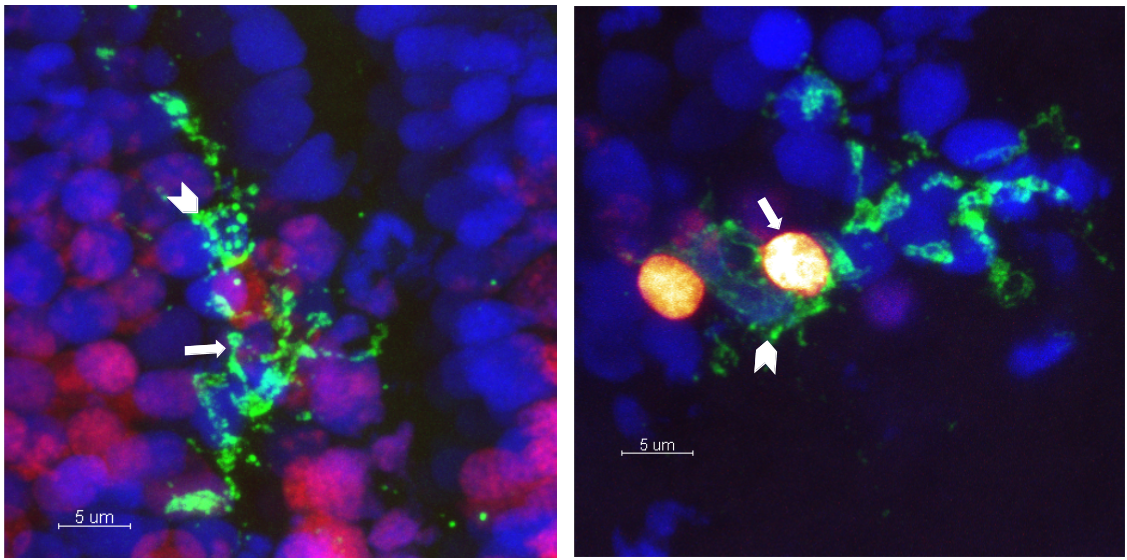
\includegraphics[width=1.\textwidth]{cmz/4C4engulfment.png}}    
    \caption{{\bf 4C4+ microglia associate with and engulf EdU-labelled CMZ contributions in the specified neural retina}}
    Representative maximum intensity projections from confocal micrographs of 14\si{\micro\metre} coronal cryosections through 30dpf zebrafish eyes labelled at 23dpf with EdU.
    
    Blue: Hoechst 33258 nuclear counterstain. Green: Microglia labelled with 4C4 antibody. Red-orange-yellow: Intensity scale of EdU staining, indicating cellular origin in the 23dpf CMZ.

    Chevrons: microglial nuclei. Arrows: EdU-positive nuclei found within 4C4-labelled extent of microglial cell body and appendages.
    
    Methods in \autoref{ssec:CMZ4C4histo}.
    \label{CMZ4C4micrograph}
\end{figure}

\begin{table}[!ht]
    \centering
    \caption{{\bf GMC-NS evidence estimates confirm Empirical Bayes analysis of early cohort stability}}
    \begin{tabular}{|l|l|l|l|l|} \hline 
        {\bf Cohort} & {\bf Time-constant logZ} & {\bf Time-varying logZ} & {\bf logZR} & {\bf $\sigma$ Significance}\\ \hline
        Embryonic central remnant & {\bf -857.08 ± 0.29} & -868.02 ± 0.6 & 10.94 ± 0.67 & 16.4\\ \hline
        1 month CMZ & {\bf -402.38 ± 0.31} & -405.76 ± 0.43 & 3.39 ± 0.53 & 6.4\\ \hline
    \end{tabular}
    \begin{flushleft} logZ: logarithm of p(D), the marginal likelihood of the data, or model evidence. logZR: evidence ratio; positive ratios in favour of the 2-phase model. Largest evidence value bolded.
    Methods in \autoref{ssec:CMZEdU}, \autoref{ssec:GMCev}.
    Code in \autoref{ssec:a27GMC_NS}.
    \end{flushleft}
    \label{turnoverGMCtable}
\end{table}

\section{Summary: Modelling the postembryonic CMZ}
CMZ population dynamics, as encapsulated in our datasets, are best explained by a model of slowly decaying cell cycle rate and constant niche exit rate. This parameterisation is superior to phased models of CMZ activity, although both imply an initial period characterised by CMZ population growth, followed by a second phase of during which the CMZ is depleted. These dynamics can be achieved with a a wide range of cycle times and niche exit rates, which we show by establishing posterior distributions on these parameters. These demonstrate that our estimates of cell cycle lengths are better constrained by our data than estimates of exit rates. The population of the CMZ displays an asymmetric structure which reverses over time; we have shown this is not due to time-shifting of the two proliferative phases across anatomical axes, nor can it be explained by different initial cell cycle times and decay rates. The proportional layer composition of CMZ-driven contributions is stable over this time, and does not display variability over the dorso-ventral axis. However, by estimating the evidence for time-stable and time-varying models of lineage contribution, we identified a decline in particular retinal lineage subtypes, particularly those of the INL, but including the GCL. This a potential explanation for the teleost postembryonic change in retinal mosaic pattern. Finally, we have shown that microglia-mediated turnover of retinal neurons is occurring at a rate too low to have a measurable effect on cohort sizes during this time.

Thus, the niche history of the CMZ is not adequately explained by a ``frozen'' population of RPC progenitors, homeostatically recapitulating a program of development found in embryonic progenitors, as has been suggested previously \cite{Harris1998,Wan2016}, for the proliferative potential implied by these models is too low. Instead, a model that does not limit the size of lineages, but has a slowly decaying cell cycle rate, is sufficient to produce the observed niche population history. This suggests that the postembryonic CMZ is under a separate regulatory regime from the embryonic RPCs, which contribute the central, larval remnant of the neural retina. This period of RPC activity benefits from separate modelling and investigation. Moreover, the decaying cycle rate model suggests an explanation for the difference between animals that have sustained CMZ RPC activity in adulthood, like teleosts, versus those that do not, such as mammals: the rate of decay in mammals may simply be much higher.

In addition to discovering unique features of postembryonic CMZ activity, we have proved out a general framework for Bayesian evaluation and selection of arbitrary biological models, which can inform both future experiments as well as modelling and theoretical choices. For instance, slice models more successfully combine population and morphological information, to answer questions about CMZ population structure, than do abstract whole-population models of the CMZ. From the foregoing analyses, we conclude that treating the CMZ population as a combined unit with shared proliferative parameter evolution is likely well justified, suggesting that much of the apparent complexity of the niche's population history can be usefully abstracted away.

\section{Future directions}
These studies show that the simple datasets we have collected are sufficient to suggest a general model of the postembryonic CMZ, which does not explicitly limit the proliferative potential of RPCs by a measure of time in lineage, like the SMME models. However, they also reveal that these datasets provide little constraint on many important parameters of interest. This is an important insight, as future experiments can be designed with the nested sampling model comparison in mind. For instance, our models consistently exhibit poorly constrained niche exit rates. The kinetics of niche exit could be examined by thymidine pulse-chase assays, timed to catch cohorts of RPC progeny as they cross the boundary from the CMZ into the neural retina, and this would likely significantly improve our estimates. Cell-based models of cycle parameters can glean some information from cumulative thymidine analogue labelling alone, but these would be greatly improved with costaining for markers of other cycle phases, for instance using phosphorylated histone H3 as a marker of M phase \cite{Ren2018}. Experiments using multiple different thymidine analogue labels \cite{Harris2018} are another avenue for refining these estimates.

In general, the model comparison approach worked out here seems promising for testing competing explanations for observed phenomena. It would be worthwhile to improve the accuracy of \hyperref[chap:GMC]{\path{GMC_NS.jl}}, and to continue developing models that make reference to the widest available array of observations and interventions. Given some adjustments to the experimental approach, and a refined sampler, this approach could replace obsolete models of cell cycle like the one described by Nowakowski et al. \cite{Nowakowski1989}, while giving a more realistic picture of the information actually provided by particular datasets.

As a final remark, it should be emphasized that the conclusions of this chapter always refer to the quality distribution jointly implied by the model and the data. Despite our failure to distinguish between RPC behaviours in different morphological regions of the CMZ, these rejected hypotheses should be returned to and re-tested with refined models and datasets. The same is true of phased and single-regime models of RPC cell cycle regulation. By proceeding in this manner, as Feyerabend suggested, we can ``maximise the empirical content of [our] views" by ``try[ing] to improve rather than discard the views that have failed in the competition.'' \cite[p.20]{Feyerabend1993}